\documentclass{article}
\usepackage{amsmath}
\usepackage{graphicx}
\usepackage{float}
\usepackage{fancyhdr}
\usepackage[spanish]{babel}
\usepackage[utf8]{inputenc}
\usepackage[justification=centering]{caption}
\usepackage[font={small}]{caption}

\parindent 0em
\parskip 2ex
\pagestyle{fancy}
\setlength{\textfloatsep}{5pt}

\begin{document}

\begin{titlepage}
\newcommand{\HRule}{\rule{\linewidth}{0.5mm}}

\center
\textsc{\LARGE ITESO, Universidad Jesuita De Guadalajara}\\[2cm]
\textsc{\Large INGENIERÍA FINANCIERA}\\[1cm]
\textsc{\large Innovación y Gestión De Proyectos}\\[1cm]
\HRule \\[2cm]
{ \huge \bfseries Accidentes viales en la Zona Metropolitana de Guadalajara}\\[2cm]
\HRule \\[2cm]
\begin{minipage}{0.4\textwidth}
\begin{flushleft} \large


\emph{Autores:}\\
\small Alicia Karime González Beltrán\\
\small Ana Goretti Chávez Flores\\
\small Rodrigo Hernández Mota\\
\small José Felipe Sánchez Andaluz
\end{flushleft}
\end{minipage}
~
\begin{minipage}{0.4\textwidth}
\begin{flushright} \large
\emph{Supervisor:} \\
\small Mtra. Mireya \textsc{Pasillas Torres}
\end{flushright}
\end{minipage}\\[2cm]

{\large \today}\\[1cm]

\vfill
 
\end{titlepage}
\tableofcontents
\newpage

\section{Introducción}\label{sec:into}
[agregar contenido]

\newpage
\section{Diagnóstico}\label{sec:diagnostic}

Datos provenientes de la Secretaría de Movilidad de Jalisco (SEMOV) señalan que en 2016 se generaron más de \textbf{23,753 accidentes viales} dentro de la zona metropolitana de guadalajara (ZMG). Esta cifra corresponde al 93\% de todos los accidentes viales de todo el estado. Aunado a esto, el INEGI reporta 3,429,847 vehículos en circulación en el estado durante este mismo año. Esto significa que de cada 1000 vehículos se generaron 7 accidentes viales en promedio. 


Es imperativo señalar que los accidentes automovilísticos se caracterizan por provocar fuertes
repercusiones económicas para los involucrados. Adicionalmente, cifras publicadas por la
Asociación Mexicana de Instituciones de Seguros (AMIS) indican que solo el 27\% del parque vehicular en
México está asegurado. Esto representa un fuerte riesgo financiero potencial para la población con
vehículo en circulación.

El estado de Jalisco, reconociendo la importancia de atender este problema,
ha realizado acciones para disminuir el número de accidentes viales.
Las políticas y soluciones que se han implementado muestran un efecto deseable en el cual
se percibe un decrecimiento real en el número de accidentes (dado que el parque vehicular ha aumentado
durante el mismo periodo de tiempo). A continuación se muestra una gráfica con el número
de accidentes viales total por año dentro de la ZMG.

	\begin{figure}[H]\centering
	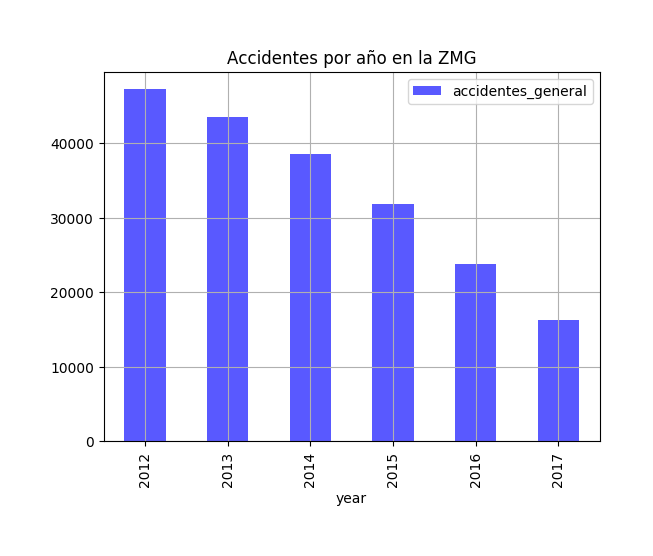
\includegraphics[width=0.60\textwidth]{resources/img/accidentes_general_img.png}
	\caption{\label{fig:accidentes_general_img} Número de accidentes viales por año dentro de la zona metropolitana de Guadalajara. Fuente: adaptación de datos de SEMOV.}
    \end{figure}

Estas políticas muestran un rendimiento excepcional en la reducción de muertes ocasionados por consumo de bebidas alcoholicas,
en donde el efecto más significativo se puede apreciar en el último año de la serie de tiempo.


	\begin{figure}[H]\centering
	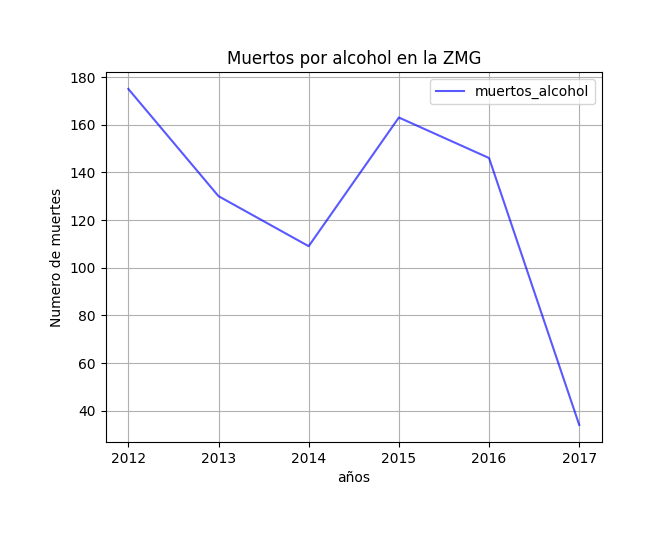
\includegraphics[width=0.60\textwidth]{resources/img/muertos_alcohol_img.png}
	\caption{\label{fig:accidentes_general_img} Número de muertes por consumo de bebidas alcoholicas dentro de la zona metropolitana de Guadalajara. Fuente: adaptación de datos de SEMOV.}
    \end{figure}


Al analizar otras variables, es posible detectar que en general la tendencia ha sido negativa.
En particular, es de especial interés mostrar la evolución del numero de accidentes por las
categorías de lesionados involucrados, muertes total, y muertes en lugar de accidente.

	\begin{figure}[H]\centering
	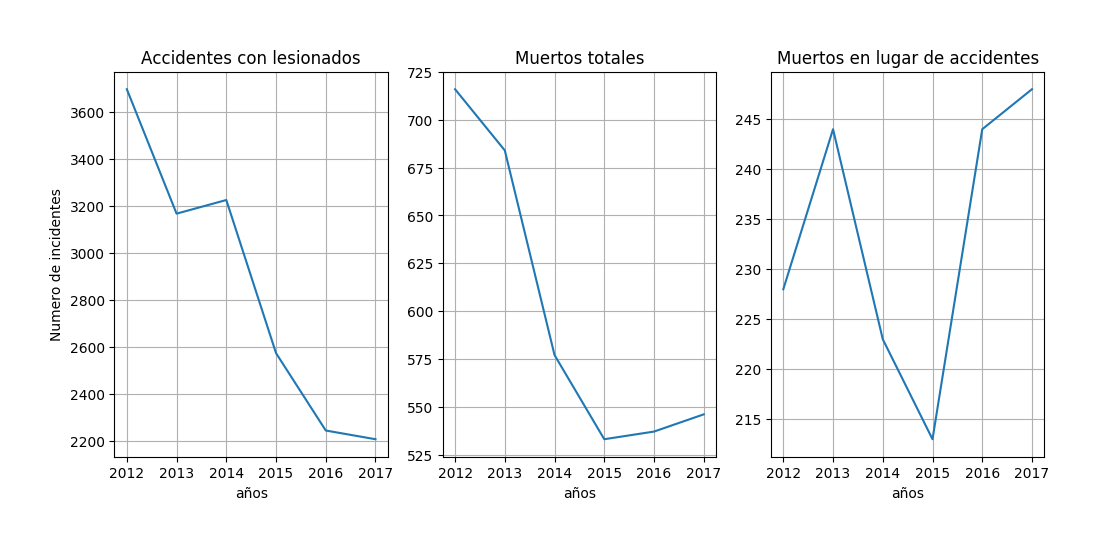
\includegraphics[width=1\textwidth]{resources/img/accidentes_general_segregacion_img.png}
	\caption{\label{fig:accidentes_general_segregacion_img} Segregación de accidentes viales dentro de la ZMG por lesionados, muertos y muertos en el lugar de accidente. Fuente: adaptación de datos de SEMOV.}
    \end{figure}

Aunque el número total de accidentes ha disminuido en forma significativa,
no todos los niveles de segregación que lo conforman presentan una disminución.
Adquiere relevance identificar en qué segmentos la actual política de SEMOV presenta
resultados deseables y aquellos cuya situación es inmune a estas políticas.
En este caso, se puede observar que el número de muertes en el lugar del accidente
vial ha incrementado de forma alarmante. Las causas de esto pueden variar desde
velocidad de reacción de servicios médicos, condiciones del impacto, muerte instantanea,
etc.

Una auditoría sobre la seguridad vial en la ZMG realizada por la SEMOV en colaboración con la Universidad de Guadalajara
identifican que entre los problemas de seguridad relevantes se encuentran:

	\begin{itemize}
		\item Desgaste natural del balizamiento.
		\item Falta de señales viales o en mal estado.
		\item Insuficientes espacios destinados a la circulación peatonal.
	\end{itemize}

Por otra parte, la SEMOV en su reporte "Zonas de Riesgo" clasifica las causas de accidente viales en:

	\begin{itemize}
		\item Falta de distancia de seguridad.
		\item Invadir carril contrario.
		\item Virar indebidamente.
		\item No respetar señalamiento.
		\item No respetar semáforos.
		\item Exceder límites de velocidad.
		\item Rebaso indebido.
		\item Falla mecánica del vehículo.
		\item Exceso de carga o dimensiones.
		\item Circular en sentido contrario.
		\item Falta de señalamiento.
		\item Dormitar.
	\end{itemize}


Este estudio prone el siguiente árbol de problemas (véase Figura \ref{fig:arbol}) con el fin de identificar las causas y consecuencias que desencadena el tema del presente de forma precisa.


	\begin{figure}[H]\centering
	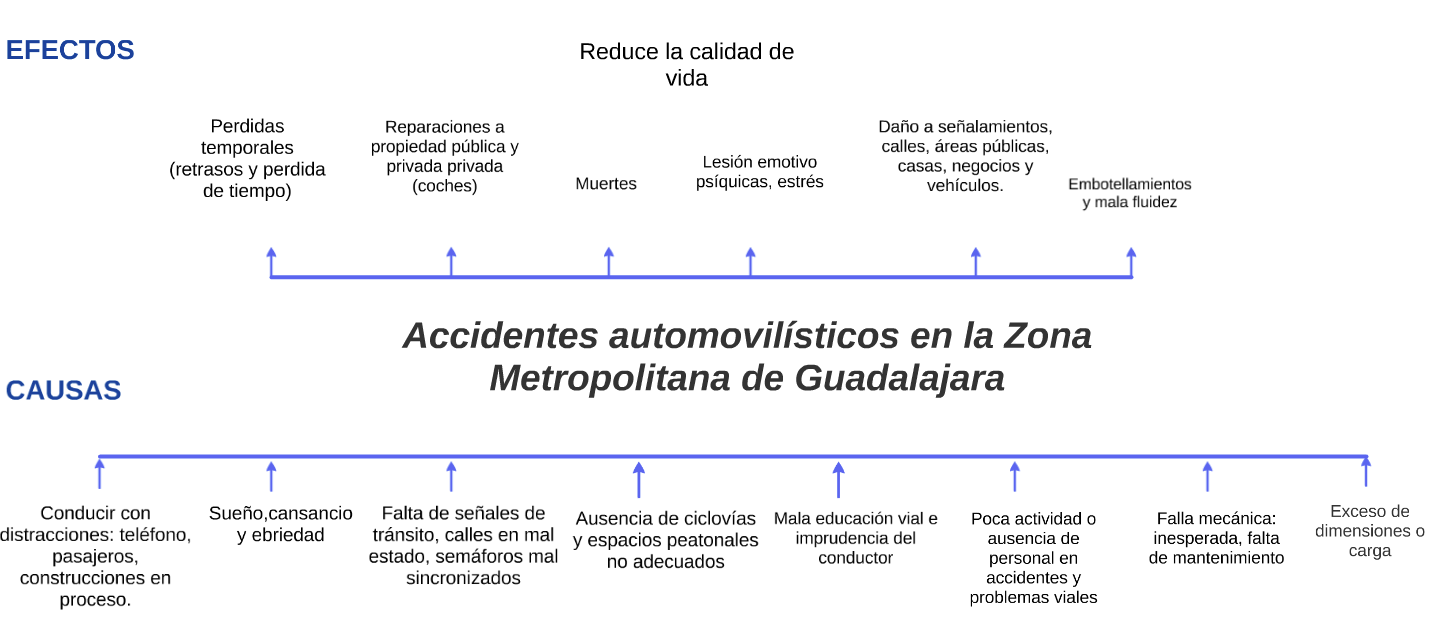
\includegraphics[width=1.25\textwidth]{resources/img/arbol_de_problemas.png}
	\caption{\label{fig:arbol} Árbol de problemas}
    \end{figure}

\newpage
\section{Objetivos del proyecto}\label{sec:objs}
[agregar contenido]

\subsection{Objetivos general}\label{subsec:general-objs}
[agregar contenido]

\subsection{Objetivos específico}\label{subsec:specific-objs}
[agregar contenido]

\newpage
\section{Análisis de los participantes}\label{sec:participants}
[agregar contenido]

\newpage
\section{Alternativas de solución}\label{sec:alternatives}
[agregar contenido]

\newpage
\section{Elaboración de la MIR}\label{sec:mir}
[agregar contenido]

\newpage
\section{Conclusiones}\label{sec:conclutions}
[agregar contenido]

\newpage
\section{Bibliografía}\label{sec:references}
[agregar contenido]

\end{document}
